\section{Stageplot}
\begin{center}
    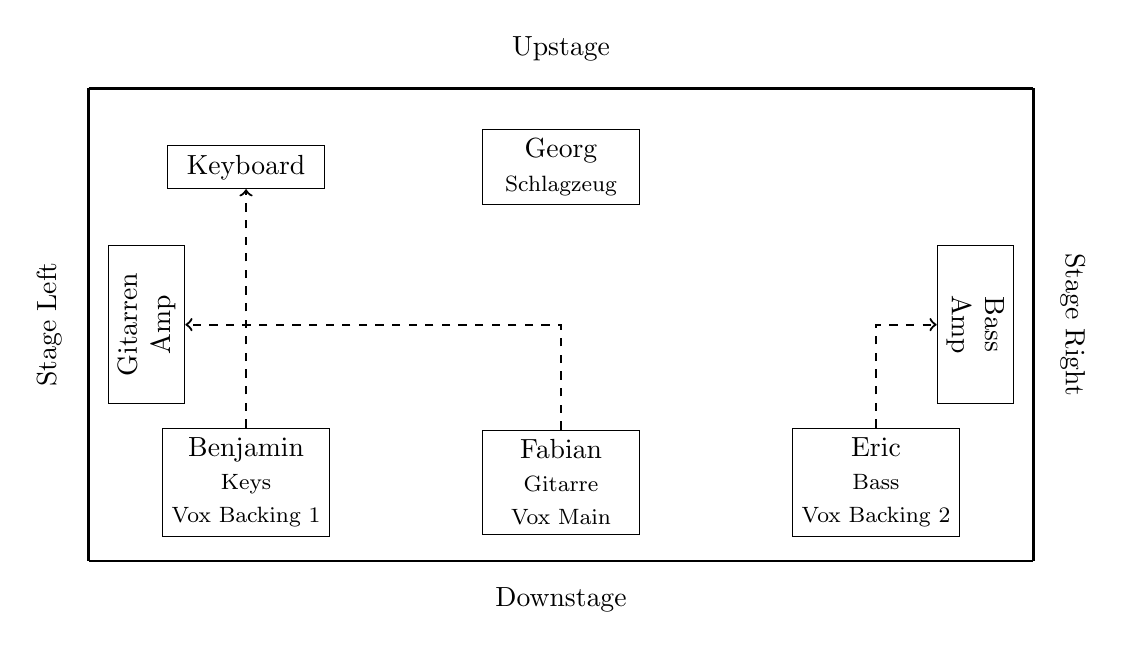
\begin{tikzpicture}[every node/.style={align=center}]    
    % Stage boundaries (Koordinaten angepasst)
    \draw[thick] (-6, -3) -- (6, -3); % Downstage
    \draw[thick] (-6, 3) -- (6, 3); % Upstage
    \draw[thick] (-6, -3) -- (-6, 3); % Stage left
    \draw[thick] (6, -3) -- (6, 3); % Stage right
    
    % Labels for stage
    \node[rotate=90] at (-6.5, 0) {Stage Left};
    \node[rotate=-90] at (6.5, 0) {Stage Right};
    \node at (0, -3.5) {Downstage};
    \node at (0, 3.5) {Upstage};
    
    % Downstage (Benjamin, Fabian, Eric)
    \node[draw, rectangle, minimum width=2cm, align=center] (benjamin) at (-4, -2) {Benjamin \\ \footnotesize Keys \\ \footnotesize Vox Backing 1};
    \node[draw, rectangle, minimum width=2cm, align=center] (fabian) at (0, -2) {Fabian \\ \footnotesize Gitarre \\ \footnotesize Vox Main};
    \node[draw, rectangle, minimum width=2cm, align=center] (eric) at (4, -2) {Eric \\ \footnotesize Bass \\ \footnotesize Vox Backing 2};
    
    % Upstage (Georg and Keyboard)
    \node[draw, rectangle, minimum width=2cm, align=center] (georg) at (0, 2) {Georg \\ \footnotesize Schlagzeug};
    \node[draw, rectangle, minimum width=2cm, align=center] (keyboard) at (-4, 2) {Keyboard};
    
    % Amplifiers
    \node[draw, rectangle, minimum width=2cm, align=center, rotate=-90, anchor=north] (bassamp) at (5.75, 0) {Bass \\ Amp};
    \node[draw, rectangle, minimum width=2cm, align=center, rotate=90, anchor=north] (guitaramp) at (-5.75, 0) {Gitarren \\ Amp};
    
    % Connections/relationships
    \draw[->, thick, dashed] (fabian.north) -- (0,0) -- (guitaramp.south);
    \draw[->, thick, dashed] (eric.north) -- (4,0) -- (bassamp.south);
    \draw[->, thick, dashed] (benjamin.north) -- (keyboard.south);
    \end{tikzpicture}
\end{center}